\documentclass{JAC2003}

%%
%%  This file was updated in April 2009 by J. Poole to be in line with Word tempaltes
%%
%%  Use \documentclass[boxit]{JAC2003}
%%  to draw a frame with the correct margins on the output.
%%
%%  Use \documentclass[acus]{JAC2003}
%%  for US letter paper layout
%%

\usepackage{graphicx}
\usepackage{booktabs}

% Newly added package
\usepackage{amsmath}
\usepackage{algorithm,algorithmic}
\usepackage{tikz}
\usepackage{multirow}
\usepackage{graphicx}
\usepackage{url}
\usepackage{cite}
\usetikzlibrary{shapes,arrows}
%%
%%   VARIABLE HEIGHT FOR THE TITLE BOX (default 35mm)
%%

\setlength{\titleblockheight}{27mm}

\begin{document}
\title{A FIELD EMISSION AND SECONDARY EMISSION MODEL IN OPAL}

\author{C. Wang, A. Adelmann, Y. Ineichen, PSI, Villigen, Switzerland}

\maketitle

\begin{abstract}
   Dark current and multipacting phenomena, as observed in accelerator
structures, are usually harmful to the equipment and the beam quality.
These effects need to be suppressed to guarantee stable operation. Large scale
simulations can be used to understand the cause and develop solutions for these
phenomena. 
We extend OPAL\cite{OP}, a parallel framework for charged particle
optics in accelerator structures and beam lines, with the necessary physics models
to simulate multipacting phenomena. This is achieved by adding a Fowler-Nordheim
field emission model and a secondary emission model, as well as 3D boundary
geometry handling capabilities to OPAL. 
With these capabilities we can evaluate dark current and multipacting in
high-gradient linac structures and in RF cavities of high intensity Cyclotrons.
In state of the art accelerator structures the electric fields are strong,
therefor space charge effects in the Fowler-Nordheim model cannot be neglect. In
a first step we add the Child-Langmuir model to phenomenologically model space
a charge limited field emission. In the near future a multigrid preconditioned
iterative space charge solver capable of handling complicated boundary
geometries will be used to make our field emission model more self-consistent.
\end{abstract}

\section{INTRODUCTION}

Dark current and multipacting phenomena have been observed in various RF
structures of accelerators, e.g. \cite{DE}\cite{CY}. These phenomena are usually
harmful to the equipment and beam quality, as they will cause galvanic
etching on the surface of the cavity and thus cause RF breakdown. In this paper
we will discuss our efforts to extend OPAL in order to get a feasible tool
for performing large scale dark current and multipacting simulations. This would
allow more thorough analysis and a deeper understanding of these phenomena.
Accurate simulations could lead to methods how these situations can be prevented
or diminished. 
To achieve these goals, first we introduce a particle-boundary collision test
model into OPAL to facilitate the particle searching during tracking process. In
a subsequent step we add surface physics models including an analytic
Fowler-Nordheim field emission model and a phenomenological secondary emission
model to OPAL.

The Child-Langmuir space charge model for emitted electrons is discussed here. A
multigrid preconditioned iterative space charge solver able to treat
complicated boundaries with higher accuracy is still work in progress and will
be incorporated in the near future.

A code benchmark of the implemented secondary emission model and visualization
results are given in the last section of the paper.

\section{PARTICLE-BOUNDARY COLLISION TEST MODEL IN OPAL}

Testing particle-boundary collisions is crucial to both dark current and
multipacting simulations. We need an efficient way to distinguish between dark
current particles potentially reaching the beam diagnostic equipment (e.g. a
screen) and those hitting the surface of beam line elements causing
multiplication.

The particle-boundary collision test in a 3D geometry is complicated and
computational expensive. Our complex 3D geometries are hard to parameterized
by simple functions. Instead we represent geometries as triangulated surface
meshes. Subsequently we can make use of efficient 3D line segment-triangle
intersection (LSTI) tests to find particle-boundary collisions. In the following
we will describe how we implemented this collision tests while still retaining
code efficiency.

\subsection{The Line Segment-Triangle Intersection (LSTI) Test}

An efficient LSTI test algorithm is described in \cite{FA}. Since we need to
precompute all triangle normals for triangle orientation anyway we can make use
of a faster algorithm relaying on having triangle normals available \cite{LT}.
In order to compute a LSTI we need the starting and end point of the
line segment under consideration, triangle vertices and normal. A schematic view
is sketched in Figure \ref{fig:L-T}.
%
\begin{figure}
\begin{center}
\scalebox{0.7}{
\begin{tikzpicture}
\usetikzlibrary{arrows}
\draw [->,black,-latex] (-1.5,0) -- (1.5,0);
\draw [->,black,-latex] (-1.5,0) -- (-1.5,2);
\draw (1.5,0) -- (0.0,2);
\draw  [<-,black,latex-](0.0,2) -- (-1.5,0.0);
\draw [->,black,-latex,dashed] (-1.5,0) -- (0.5,0.5);
\node[below] (w) at (-0.15,0.5) {$\vec{w}$};
\draw[dashed] (0.5,0.5) -- (-1.18,0.5);
\draw[dashed] (0.5,0.5) -- (0.01,0.0);
\node[above] (ti) at (-1.18,0.5) {$t_i$};
\node[below] (si) at (0.01,0.0) {$s_i$};
\node[above] (t0) at (-1.7,0.) {$\mathbf{t_0}$};
\node[right] (t1) at (1.5,0) {$\mathbf{t_1}$};
\node[above] (t2) at (0.0,2.0) {$\mathbf{t_2}$};
\node[above] (n) at (-1.5,2) {$\vec{n}$};
\node[above] (v) at (-0.5,1.5) {$\vec{v}$};
\node[below] (u) at (1.2,0.0) {$\vec{u}$};
\path[draw=black,fill=black] (0.0,2.0) circle (2pt);
\path[draw=black,fill=black] (1.5,0.0) circle (2pt);
\path[draw=black,fill=black] (-1.5,0.0) circle (2pt);
\draw (-3.5,-1) -- (2.5,-1);
\draw (2.5,-1) -- (5,3);
\draw (0,3) -- (5,3);
\draw (-3.5,-1) -- (0,3);
\draw (0.5,0.5) -- (1.6,5);
\path[draw=black] (0.5,0.5) circle (2pt);
\node[above] (I) at (0.5,0.5) {$\mathbf{I}$};
\node[right] (x0) at (1.6,5) {$\mathbf{x_0}$};
\draw[dashed] (0.5,0.5) -- (-0.1,-1.9);
\node[right] (x1) at (0.0,-1.9) {$\mathbf{x_1}$};
\node[right] (ri) at (1,2.5) {$r_i$};
\path[draw=black,fill=black] (-0.1,-1.9) circle (2pt);
\path[draw=black,fill=black] (1.6,5) circle (2pt);
\end{tikzpicture}
}
\end{center}
\caption{Line segment-triangle intersection.\label{fig:L-T}}
\end{figure}
%
Vectors are denoted with arrows (i.e. $\vec{n}$), points (here in
$\mathcal{R}^3$) are bold (i.e. $\mathbf{x}_0$) and the remaining symbols denote
scalars. The algorithm for handling LSTI is given in Algorithm \ref{alg:lsti}.
%
\begin{algorithm}
  \caption{LSTI} \label{alg:lsti}
   \begin{algorithmic}[1]
     %\STATE \textbf{procedure} LSTI(\textbf{In:} line segment $\mathbf{x}_1-\mathbf{x}_0$, $\Delta(\mathbf{t}_0, \mathbf{t}_1, \mathbf{t}_2)$, \textbf{Out:} true $ \&\ \mathbf{I}$ or false)
     \STATE \textbf{procedure} LSTI(\textbf{In:} $\mathbf{x}_0$, $\mathbf{x}_1$, $\Delta(\mathbf{t}_0, \mathbf{t}_1, \mathbf{t}_2)$, \textbf{Out:} isInside, $\mathbf{I}$)
     \IF{$\vec{n} \cdot (\mathbf{x}_1-\mathbf{x}_0)=0$}
     \RETURN false \COMMENT{$\mathbf{x}_1-\mathbf{x}_0~||~\Delta \rightarrow$ no intersection}
     \ELSE
     \STATE $ r_i \leftarrow \frac{\vec{n} \cdot (\mathbf{t}_0-\mathbf{x}_0)}{ \vec{n}\cdot(\mathbf{x}_1-\mathbf{x}_0)} $
     \STATE $\mathbf{I} \leftarrow \mathbf{x}_0+r_i(\mathbf{x}_1-\mathbf{x}_0) $ \COMMENT {The intersection point of the line segment and planed}
     \IF{$ r_i $$<$$ 0$ \textbf{or} $ r_i$ $>$ $1 $}
        \RETURN false \COMMENT{early rejection: intersection is on the extension of line segment}
     \ELSE 
        \STATE \COMMENT{Check if the intersection point is inside the triangle}
        %\STATE The parametric plane equation: $ \mathbf{t}(s_i,t_i)=\mathbf{t}_0+s_i (\mathbf{t}_1-\mathbf{t}_0)+t_i(\mathbf{t}_2-\mathbf{t}_0)=\mathbf{t}_0+s_i\vec{u}+t_i\vec{v} $. As $\vec{w}=\mathbf{I}-\mathbf{t}_0$ is also in the plane, 
        \STATE Solve: $\vec{w}=\mathbf{t}_0+s_i\vec{u}+t_i\vec{v}$ \COMMENT{parametric plane equation}
        \STATE $s_i \leftarrow \frac{(\vec{u} \cdot \vec{v})(\vec{w} \cdot \vec{v})-(\vec{v} \cdot \vec{v})(\vec{w} \cdot \vec{u})}{(\vec{u} \cdot \vec{v})^2-(\vec{u} \cdot \vec{u})(\vec{v} \cdot \vec{v})}$
        \STATE $t_i \leftarrow \frac{(\vec{u} \cdot \vec{v})(\vec{w} \cdot \vec{u})-(\vec{u} \cdot \vec{u})(\vec{w} \cdot \vec{v})}{(\vec{u} \cdot \vec{v})^2-(\vec{u} \cdot \vec{u})(\vec{v} \cdot \vec{v})}$
        \IF{$ s_i \geq 0 $ \textbf{and} $ t_i \geq 0 $ \textbf{and} $ s_i+t_i \leq 1 $} 
            \RETURN (true, $\mathbf{I}$)
        \ELSE
            \RETURN false \COMMENT{no intersection between line segment and triangle}
        \ENDIF
     \ENDIF
\ENDIF
       \STATE \textbf{end procedure}
   \end{algorithmic}
 \end{algorithm}
 \subsection{Early Rejection Strategy}
Even though the implemented LSTI algorithm using precomputed triangle normal is
fast a huge number of LSTI calls are necessary. If we have $M$ triangles and $N$
particles in the simulation, both in the magnitude of hundreds of thousand to
millions, the number of LSTI tests in single time step without a early rejection
strategy would be $M \times N$, i.e., at least $10^{10}$ per time step.
Obviously, effective early rejection strategies (see Figure~\ref{fig:P-B}) are
needed to reduce the number of LSTI tests.

\begin{figure}[H]
    \begin{center}
        
\scalebox{0.7}{
\begin{tikzpicture}
\draw[step=1cm,gray,dashed] (-3,0) grid (3,6);
\draw[step=1cm,gray,dashed,fill=gray!30] (-3,3) rectangle (-2,4); 
\draw[step=1cm,gray,dashed,fill=gray!30] (-2,1) rectangle (-1,2); 
\draw[step=1cm,gray,dashed,fill=gray!30] (-2,2) rectangle (-1,3); 
\draw[step=1cm,gray,dashed,fill=gray!30] (-2,3) rectangle (-1,4);
\draw[step=1cm,gray,dashed,fill=gray!30] (-1,1) rectangle (0,2);
\draw[step=1cm,gray,dashed,fill=gray!30] (-1,0) rectangle (0,1);
\draw[step=1cm,gray,dashed,fill=gray!30] (0,0) rectangle (1,1);
\draw[step=1cm,gray,dashed,fill=gray!30] (0,1) rectangle (1,2);
\draw[step=1cm,gray,dashed,fill=gray!30] (1,1) rectangle (2,2);
\draw[step=1cm,gray,dashed,fill=gray!30] (1,2) rectangle (2,3); 
\draw[step=1cm,gray,dashed,fill=gray!30] (1,3) rectangle (2,4);
\draw[step=1cm,gray,dashed,fill=gray!30] (2,3) rectangle (3,4);
\draw[step=1cm,gray,dashed,fill=gray!30] (-3,4) rectangle (-2,5);
\draw[step=1cm,gray,dashed,fill=gray!30] (-3,5) rectangle (-2,6);
\draw[step=1cm,gray,dashed,fill=gray!30] (2,4) rectangle (3,5);
\draw[step=1cm,gray,dashed,fill=gray!30] (2,5) rectangle (3,6);   
\draw[black, thick] (0.,0.5) parabola  ( 2.5,5.5); 
\draw[black, thick] (0.,0.5) parabola  ( -2.5,5.5);
\draw [->,gray] (-1.55,2.5) -- (-1,2.8);
\node[above] (n) at (-1,2.8) {$\vec{n}$};
\draw [<-,gray] (1.0,4.1) -- (2,3.7);
\node[above] (n) at (1,4.1) {$\vec{n}$};
%\tikz[label distance=4mm]
\draw (-1.2,2.1) node[circle,fill=yellow]{};
\draw [->,thick] (-1.2,2.1) -- (-0.3,2.1);
\draw (0,4.1) node[circle,fill=green]{};
\draw [->,thick] (0,4.1) -- (0.3,4.4);
\draw (1.2,3.5) node[circle,fill=red]{};
\draw [<-,thick] (1.8,3.5) -- (1.2,3.5);
\end{tikzpicture}
}
    \end{center}
    \caption{Schematic view of particle-boundary early rejection strategy. The dark
    black line represents the boundary surface, particles are colored dots with an
    attached momenta arrow and inward normals gray arrows.\label{fig:P-B}}
\end{figure}

Assuming we need to determine whether a particle with position $\mathbf{r}$
and momenta $\mathbf{p}$ hits the boundary within time step $\Delta{t}$ we apply
the following early rejection strategies:
\begin{itemize}
    \item Test if the particle is near the boundary by checking if $\mathbf{r}$
    is inside the boundary bounding boxes (illustrated by gray grids in
    Figure ~\ref{fig:P-B}). 
    \item If $\mathbf{r}$ is not in a bounding box (green particle in Figure
    ~\ref{fig:P-B}), the particle is enough far away from boundary and
    can be integrated directly.
    \item If $\mathbf{r}$ is in a bounding box (yellow particle and red particle
    in Figure ~\ref{fig:P-B}), then we check all triangles in the bounding box
    (of the corresponding particle) as well as triangles in the adjacent 26
    bounding boxes to see if the momenta of the particle has a opposite
    direction with those triangles' normals.
    \item If the momenta and triangle normal are not opposite for all triangles
    checked (the yellow particle) do particle integration.
    \item If they are opposite (red particle) check if the particle has an
    intersection with the triangles by performing the LSTI test for each
    triangle. If an intersection exists the particle will hit the boundary
    during the current time step.
\end{itemize}

Two things need to be pointed out. First we get the inward normal in the
following way. We find a point close to a triangle with specified ID (e.g. 0)
and determine if the point is inside or outside the boundary geometry. This can
be achieved by doing a ray-boundary intersection test and counting the number of
intersections. Using this point we can get the orientation (inward normal) of
the triangle with ID 0. Now we can get the inward normal of all
surface triangles by recursively aligning the orientation of adjacent triangles
of triangles whose inward normals have already been computed.

Secondly the success of the above particle-boundary collision test relies on the
fact that the distance a particles travel in one time step cannot be larger than
the bounding box size. Choosing an appropriated bounding box size ensures that a
particle will never jump over a bounding box in one time step.

\section{SURFACE PHYSICS MODELS}

\subsection{Field Emission Model}

Field emission is a major source of both dark current particles and primary
incident particles in secondary emission. The Fowler-Nordheim (F-N) formula
we use here to predict the emitted current density is given in (\ref{eq:units})
\cite{BC} \cite{FN}
%
\begin{equation}\label{eq:units}
    J(\mathbf{r},t) = \frac{A(\beta E)^2}{\varphi t(y)^2}
                      \exp{\left(\frac{-B v(y)\varphi^{3/2}}{\beta E}\right)}
                      \left[\hbox{A/$m^2$}\right]
\end{equation}
%
where $J(\mathbf{r},t)$ stands for emitted electric current density in position
$\mathbf{r}$ and time $t$. The Greek letters $\varphi$ and $\beta$ denote the
work function of the surface material and the local field enhancement factor
respectively. The parameter $E$ is the electric field in the normal direction
of surface. The parameters $A$ and $B$ are empirical constants. The functions
$v(y)$ and $t(y)$ representing the image charge effects \cite{BC} as a function
of the Fowler-Nordheim parameter $y$ with the following definition\cite{DE}
%
\begin{equation}\label{eq:imagecharge}
    y = \sqrt{\frac{e^3}{4\pi\varepsilon}}\frac{\sqrt{\beta E}}{\varphi} 
      = 3.795\times10^{-5}\frac{\sqrt{\beta E}}{\varphi} \text{.}
\end{equation}
%
In our model, we have choosen a simpler approximation originated by J. H. Han\cite{DE}
\begin{eqnarray*}
v(y) &=& a-by^2 \\
t(y) &\approx& 1 \text{.}
\end{eqnarray*}
These approximations are valid for a large range of $y$, corresponding to
typical applied electric field ranges in RF guns.

Users can customize dark current simulation by specifying the value of the work
function $\varphi$, local field enhancement factor $\beta$ and other parameters
present in (\ref{eq:units}) and (\ref{eq:imagecharge}) in the OPAL input file.

\subsection{Space Charge Limited Current Density}

Whenever the normal components of an electric field are strong enough the field
emission current density will be limited by space charge effect\cite{BC}. 
To cover this situation we incorporated the 1D Child-Langmuir law
%
\begin{align}\label{eq:SpaceCharge}
    J(\mathbf{r},t) & =\frac{4\varepsilon_0}{9}\sqrt{2\frac{e}{m}}\left(\frac{V^{3/2}}{d^2}\right)\notag\\
    &
    =\frac{4\varepsilon_0}{9}\sqrt{2\frac{e}{m}}\left(\frac{E^{3/2}}{d^{1/2}}\right)
    \left[\hbox{A/$m^2$}\right]
\end{align}
%
into our field emission model. $J(\mathbf{r},t)$ denotes space charge limited emission 
current density in position $\mathbf{r}$ and time $t$, $\varepsilon_0$ the
permittivity in vacuum, $E$ the normal component of electric field on the surface
and $d$ the distance from the position where $E$ is evaluated. Currently we 
choose $d$ to be equal to the distance travelled by emitted particles in one
time step, i.e., $d=\frac{eE\Delta{t}^2}{2m_0}$ where $\Delta{t}$ is simulation
time step.

A multigrid preconditioned iterative space charge solver developed by Adelmann
et al. \cite{SV} has already been implemented in OPAL. We are in the process of
adapting the solver to be able to cope with the geometric boundaries present in 
our simulations.

\subsection{Secondary Emission Model}

Our implementation of the secondary emission model is based on a
phenomenological model developed by M. A. Furman and M. Pivi\cite{SE}. This
choice was based on the self-consistency property this particular secondary
model offers. In this context self-consistency means that if we define one incident
electron and the followed secondary emission procedure as an event, the event
generator is constructed so that
%
\begin{enumerate}
    \item when averaging over an infinite number of secondary-emission events, 
    the reconstructed secondary emission yield $\delta$ and its energy spectrum
    $ d\delta/dE$ are guaranteed to agree with the corresponding input quantities 
    \item the energy integral of $d\delta/dE$ is guaranteed to equal $\delta$
    \item the energy of any given emitted electron is guaranteed not to exceed the 
    primary energy
    \item the aggregated energy of the electrons emitted in any multi-electron event 
    is also guaranteed not to exceed the primary energy.
\end{enumerate}


\begin{figure}
    \begin{center}
        %\usepackage[latin1]{inputenc}
%\usepackage{tikz}
%\usetikzlibrary{shapes,arrows}

%<
%\usepackage{verbatim}
%\usepackage[active,tightpage]{preview}
%\PreviewEnvironment{tikzpicture}
%\setlength\PreviewBorder{5pt}%
%



% Define block styles
\tikzstyle{decision} = [draw,diamond, fill=blue!20, 
    text width=4.5em, text badly centered, node distance=2.2cm, inner sep=0pt]
\tikzstyle{block} = [draw,rectangle, fill=blue!20, 
    text width=7.5em, text badly centered, inner sep=3pt, rounded corners, minimum height=4em]
\tikzstyle{line} = [draw, -latex']
\tikzstyle{cloud} = [draw, \ellipse,fill=red!20, node distance=2.2cm,
    minimum height=2em]
\tikzstyle{every node}=[font=\small]
\scalebox{0.75}{
\begin{tikzpicture}[node distance = 2.2cm, auto, every node/.style={anchor=base,font=\small}]
    % Place nodes
    \node [block] (incident) {Incident $E_0$, $\theta_0$};
   % \node [cloud, left of=incident] (expert) {expert};
   % \node [cloud, right of=incident] (system) {system};
    \node [block, below of=incident, node distance=2.2cm] (yield) {Compute $\delta_e(E_0,\theta_0)$, $\delta_r(E_0,\theta_0)$, $\delta_{ts}(E_0,\theta_0)$};
    \node [block, below of=yield, node distance=2.2cm] (probability) {Compute $P_n, n=0,1,...,M$};
    \node [block, below of=probability, node distance=2.5cm] (secondaryNum) {Random integer $n$ with probability distribution $\{P_n\}$};
    \node [decision, right of=incident, node distance=3.5cm] (decide) {$n=0$?};
    \node [block, right of=decide, node distance=3.5cm] (zero) {Delete the incident electron};
    \node [decision, below of=decide, node distance=3.0cm] (decide1) {$n=1$?};
    \node [block, right of=decide1, node distance=3.5cm] (one) {Emitted energy $E\in[0,E_0]$ with PDF $f_{1,e}+f_{1,r}+f_{1,ts}$ };	\node [block, below of=decide1, node distance=3.5cm] (ts) {Emitted energy $E_k\in[0,E_0]$, $k=1,...,n$ with PDF $f_{n,ts}$ };
    \node [block, below of=one, node distance=3.5cm] (angle) {Generate $\theta_k\in[0,\pi/2]$, with PDF $cos^{\alpha}$; and $\phi_k\in[0,2\pi]$, $k=1,...,n$. Calc momenta accordingly. };
    % Draw edges
    \path [line] (incident) -- (yield);
    \path [line] (yield) -- (probability);
    \path [line] (probability) --  (secondaryNum);		
   % \path [line] (probability) -- (secondaryNum);
   % \path [line] (decide) -- node [near start] {$No$} (secondaryNum);
    \draw[->] (secondaryNum) -| +(1.8,3) |- (decide);
    %\path [line] (decide) -- node [near start,above] {yes} (zero);
    \draw[->] (decide) -- node [midway,above=2pt] {yes} (zero);	
    \path [line] (decide) -- node [midway,right=2pt] {no} (decide1);
    \path [line] (decide1) -- node [midway,above=2pt] {yes} (one);
    \path [line] (decide1) -- node [midway,right=2pt] {no} (ts);
    \path [line] (ts) -- (angle);

    \path [line] (one) -- (angle);
    \path [line] (zero) -- +(0,1.5)-| node [near start,above=2pt] {Next event} (incident);
    \path [line] (angle) -- +(0,-2.)--  node [midway,above=2pt] {Next event} (-2,-8.65) |- (incident) ;
 %\path [line] (secondaryNum) -|- (decide);
  %  \path [line] (decide) -- node {no}(stop);
   % \path [line,dashed] (expert) -- (incident);
  %  \path [line,dashed] (system) -- (incident);
   % \path [line,dashed] (system) |- (probability);
\end{tikzpicture}
}

    \end{center}
    \caption{Basic computational procedure of secondary emission model.\label{fig:S-E}}
\end{figure}

The basic computational procedure of the secondary emission model is shown in
Figure \ref{fig:S-E}. This model calculates the number of secondary electrons
that result from an incident electron of a given energy on a material at a
given angle (see Figure~\ref{incident electrons}). For each of the generated 
secondary electrons the associated process: {\em true secondary}, {\em rediffused} or
{\em backscattered} is recorded. 

\begin{figure}[H]
    \centering
    /Users/adelmann/svnwork/adelmann/papers/figures/Latex-Figures/Incident.tikz
    % \includegraphics[width=3 in]{incident_diagram.pdf}
    \caption{Geometry used by the secondary electrons model.}
    \label{incident electrons}
\end{figure}

\section{CODE BENCHMARK AND RESULT VISUALIZATION}

\subsection{Code Benchmark on Secondary Emission Model}

In order to validate the secondary model implemented in OPAL, we conducted a
code to code comparison with the TxPhysics library \cite{TX}. The simulation
parameters were fixed to a large number of incident events (10000) with the same
energy (300eV) and the same incident angle (normal to the surface). Figure
\ref{fig:cc} shows the result of the comparison between OPAL and TxPhysics. We
note that the statistical agreement is very good.
%
\begin{figure}[H]
    \begin{center}
        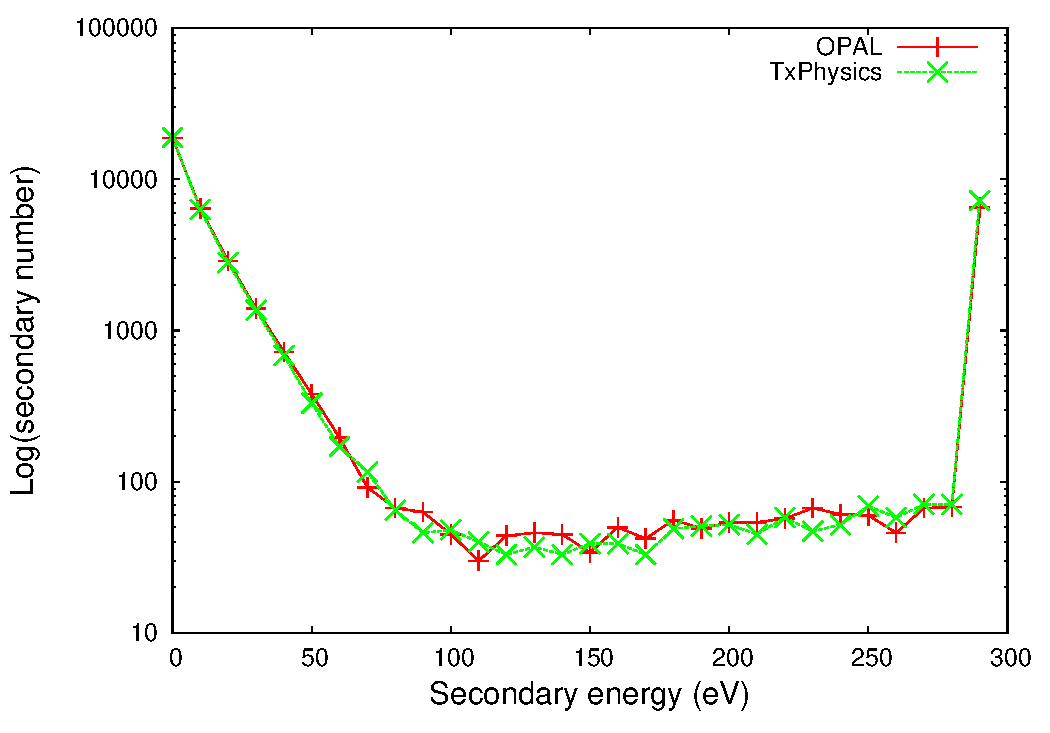
\includegraphics[width=0.5\textwidth]{code_comparison.pdf}
    \end{center}
    \caption{Secondary energy comparison between OPAL and TxPhysics.\label{fig:cc}}
\end{figure}

\subsection{Result Visualization}

For visualization purposes the boundary geometry is stored into a VTK legacy
file. Phase space data of all particles is dumped into a H5Part \cite{??}. With
a separate post processing code the H5Part particle data is converted to a VTK
legacy file At this point the VTK files can be visualized by tools like        .
Paraview\cite{PR} . A sample visualization of a dark current simulation result
is shown in Figure \ref{fig:vi}.
%
\begin{figure}[H]
\begin{center}
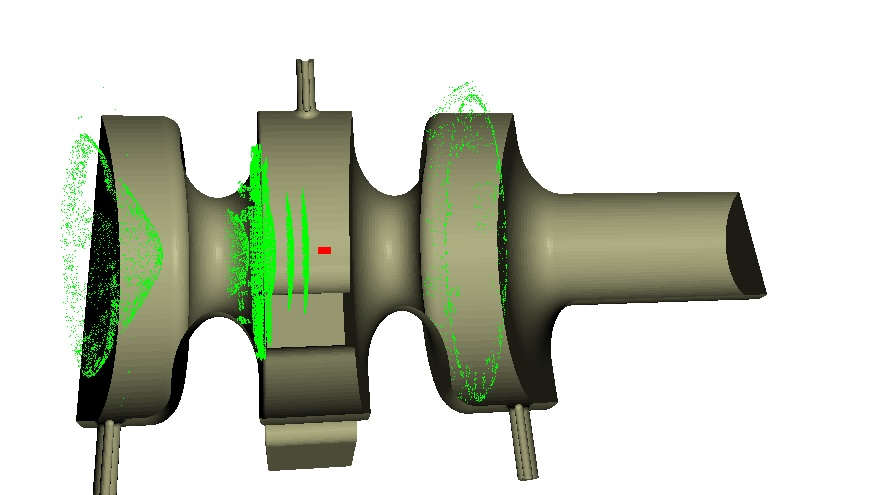
\includegraphics[width=0.4\textwidth]{newgun.jpg}
\end{center}
\caption{Simulation visualization. Dark current (green) and bunch (red)
particles inside PSI XFEL gun.\label{fig:vi}}
\end{figure} 


\begin{thebibliography}{9}   % Use for  1-9  references
%\begin{thebibliography}{99} % Use for 10-99 references
\bibitem{OP} A. Adelmann and Ch. Kraus and Y. Ineichen and  J. Yang,
The OPAL (Object Oriented Parallel Accelerator Library) 
              Framework, Paul Scherrer Institute, PSI-PR-08-02, 2008
\bibitem{DE} J. H. Han, PhD Thesis, Desy, 2005 Available Online on \url{http://www-library.desy.de/preparch/desy/thesis/desy-thesis-05-045.pdf}
\bibitem{CY} P. K. Sigg, Reliability of High Beam Power Cyclotron RF-Systems at PSI, 
Proceedings of the Workshop on Utilization and Reliability of High Power Proton Accelerators: Aix-en-Provence, France, 22-24 November 1999. Available Online on: \url{http://rf.web.psi.ch/files/proceedings/1998/JAERI98/PaperNEA98.pdf}.
\bibitem{FA} T. M\"oller and B. Trumbore,
 ACM SIGGRAPH 2005 Courses, July 31-August 04, 2005, Los Angeles, California   [doi:10.1145/1198555.1198746] 
\bibitem{LT} D. Sunday,
 Available Online on: \url{http://softsurfer.com/Archive/algorithm_0105/algorithm_0105.htm}
\bibitem{BC} Y. Feng and J. P. Verboncoeur,
Phys.Plasmas 13, 073105 (2006)
\bibitem{FN} R. H. Fowler and L. Nordheim, 
Proc. R. Soc. London, Ser. A 119, 173 (1928)
\bibitem{SV} A. Adelmann, P. Arbenz and Y. Ineichen, 
J. Comp. Phys, 229 (12): 4554-4566 (2010)
\bibitem{SE} M. A. Furman and M. T. F. Pivi,  
Phys. Rev. ST Accel. Beams 5, 124404 (2002)
\bibitem{TX}TxPhysics Users Manual, \url{http://txphysics.txcorp.com}
\bibitem{PR}A. Henderson, ParaView Guide, A Parallel Visualization Application.
Kitware Inc., 2007. \url{http://www.kitware.com/products/paraview.html}
\end{thebibliography}

\end{document}
